\documentclass[10pt,a4paper]{article}

\usepackage[utf8]{inputenc}
\usepackage[T1]{fontenc}
% \usepackage[french]{babel} % Removed - not available
\usepackage[margin=1.5cm]{geometry}
\usepackage{amsmath,amssymb}
\usepackage{xcolor}
\usepackage{tcolorbox}
\tcbuselibrary{breakable}
\usepackage{listings}
\usepackage{hyperref}
\usepackage{tikz}
\usetikzlibrary{positioning,calc,arrows.meta,shapes.geometric}

\lstset{
    language=bash,
    basicstyle=\ttfamily\scriptsize,
    backgroundcolor=\color{gray!10},
    keywordstyle=\color{blue},
    commentstyle=\color{gray},
    stringstyle=\color{red},
    numbers=left,
    numberstyle=\tiny,
    breaklines=true,
    frame=single,
    showstringspaces=false,
    tabsize=4,
    inputencoding=utf8,
    extendedchars=true,
    literate={é}{{\'e}}1 {è}{{\`e}}1 {à}{{\`a}}1 {ç}{{\c{c}}}1 
             {ê}{{\^e}}1 {î}{{\^i}}1 {ô}{{\^o}}1 {û}{{\^u}}1 {ù}{{\`u}}1
             {É}{{\'E}}1 {È}{{\`E}}1 {À}{{\`A}}1 {Ç}{{\c{C}}}1
             {Ê}{{\^E}}1 {Î}{{\^I}}1 {Ô}{{\^O}}1 {Û}{{\^U}}1 {Ù}{{\`U}}1
             {ë}{{\"e}}1 {ï}{{\"\i}}1 {ö}{{\"o}}1 {ü}{{\"u}}1
             {Ë}{{\"E}}1 {Ï}{{\"I}}1 {Ö}{{\"O}}1 {Ü}{{\"U}}1
             {œ}{{\oe}}1 {Œ}{{\OE}}1 {æ}{{\ae}}1 {Æ}{{\AE}}1
}

\newtcolorbox{infobox}[1]{
    colback=blue!5,colframe=blue!75!black,
    fonttitle=\bfseries,title=#1,breakable
}

\newtcolorbox{exercicebox}[1]{
    colback=green!5,colframe=green!50!black,
    fonttitle=\bfseries,title=#1,breakable
}

\newtcolorbox{warningbox}[1]{
    colback=red!5,colframe=red!75!black,
    fonttitle=\bfseries,title=#1,breakable
}

\newtcolorbox{techbox}[1]{
    colback=orange!5,colframe=orange!75!black,
    fonttitle=\bfseries,title=#1,breakable
}

\title{\textbf{TP-1 : Setup Environnement de Développement}\\
\large Installation Docker et Configuration}
\author{Dr. El Hadji Bassirou TOURÉ\\
Département de Mathématiques et Informatique\\
Faculté des Sciences et Techniques\\
Université Cheikh Anta Diop de Dakar}
\date{}

\begin{document}

\maketitle

\section*{Introduction}

Ce TP couvre l'installation et la configuration de l'environnement Docker standardisé pour le cours de Programmation C Avancée. Tous les TP du semestre utiliseront cet environnement pour garantir la cohérence et la reproductibilité.

\begin{infobox}{Pourquoi Docker ?}
Docker garantit que tous les étudiants travaillent dans un environnement identique, indépendamment de leur système d'exploitation (Windows, macOS, Linux). Cela évite les problèmes de "ça marche sur ma machine" et facilite le support technique.
\end{infobox}

\begin{center}
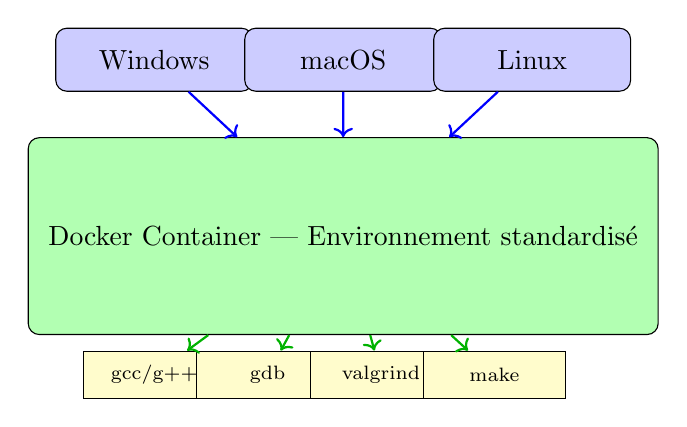
\begin{tikzpicture}[scale=0.8,
    os/.style={rectangle,rounded corners,draw,fill=blue!20,minimum width=2.5cm,minimum height=0.8cm,align=center},
    docker/.style={rectangle,rounded corners,draw,fill=green!30,minimum width=8cm,minimum height=2.5cm,align=center},
    tool/.style={rectangle,draw,fill=yellow!20,minimum width=1.8cm,minimum height=0.6cm,align=center,font=\scriptsize}]

\node[os] (win) at (0,0) {Windows};
\node[os] (mac) at (3,0) {macOS};
\node[os] (lin) at (6,0) {Linux};

\node[docker] (dock) at (3,-2.8) {Docker Container --- Environnement standardisé};

\node[tool] (gcc) at (0,-5) {gcc/g++};
\node[tool] (gdb) at (1.8,-5) {gdb};
\node[tool] (val) at (3.6,-5) {valgrind};
\node[tool] (make) at (5.4,-5) {make};

\draw[->,thick,blue] (win) -- (dock);
\draw[->,thick,blue] (mac) -- (dock);
\draw[->,thick,blue] (lin) -- (dock);

\draw[->,thick,green!70!black] (dock) -- (gcc);
\draw[->,thick,green!70!black] (dock) -- (gdb);
\draw[->,thick,green!70!black] (dock) -- (val);
\draw[->,thick,green!70!black] (dock) -- (make);

\end{tikzpicture}
\end{center}

\section*{Objectifs}

À la fin de ce TP, vous serez capable de:
\begin{itemize}
\item Installer Docker sur votre système d'exploitation
\item Télécharger et exécuter l'image Docker du cours
\item \textbf{Utiliser Vim pour créer et éditer des fichiers C}
\item Compiler et exécuter un programme C simple
\item Utiliser les outils de base (gcc, gdb, make)
\item Partager des fichiers entre votre système et le container
\end{itemize}

\begin{warningbox}{Prérequis essentiel}
\textbf{La maîtrise de Vim est un prérequis pour tous les TP suivants.} Prenez le temps de faire tous les exercices Vim de ce TP. Vous utiliserez Vim dans chaque session de travail du cours.
\end{warningbox}

\section{Prérequis Système}

\begin{techbox}{Configuration minimale}
\textbf{Matériel:}
\begin{itemize}
\item Processeur: x86\_64 (Intel/AMD) ou ARM64 (Apple Silicon)
\item RAM: 4 GB minimum, 8 GB recommandé
\item Espace disque: 10 GB disponibles
\end{itemize}

\textbf{Systèmes d'exploitation supportés:}
\begin{itemize}
\item Windows 10/11 (64-bit, avec WSL2)
\item macOS 10.15 (Catalina) ou plus récent
\item Linux: Ubuntu 20.04+, Debian 10+, Fedora 32+, etc.
\end{itemize}
\end{techbox}

\section{Installation de Docker}

\subsection{Windows}

\begin{exercicebox}{Installation Docker Desktop sur Windows}
\textbf{Étape 1: Activer WSL2}

Ouvrir PowerShell en mode administrateur et exécuter:
\begin{verbatim}
wsl --install
\end{verbatim}

Redémarrer le système après l'installation.

\textbf{Étape 2: Télécharger Docker Desktop}

Aller sur \url{https://www.docker.com/products/docker-desktop/}

Télécharger "Docker Desktop for Windows".

\textbf{Étape 3: Installer}

Exécuter l'installeur et suivre les instructions.

Cocher l'option "Use WSL 2 instead of Hyper-V".

Redémarrer après l'installation.

\textbf{Étape 4: Vérifier}

Ouvrir un terminal (Git Bash recommandé, ou PowerShell) et taper:
\begin{verbatim}
docker --version
docker run hello-world
\end{verbatim}

Si vous voyez le message de bienvenue de Docker, l'installation a réussi.
\end{exercicebox}

\begin{warningbox}{Problèmes courants Windows}
\textbf{Erreur "WSL 2 installation is incomplete":}
\begin{verbatim}
wsl --update
wsl --set-default-version 2
\end{verbatim}

\textbf{Erreur de virtualisation:}
Activer la virtualisation dans le BIOS (VT-x pour Intel, AMD-V pour AMD).

\textbf{Docker Desktop ne démarre pas:}
Vérifier que les services WSL sont actifs dans les services Windows.
\end{warningbox}

\subsection{macOS}

\begin{exercicebox}{Installation Docker Desktop sur macOS}
\textbf{Étape 1: Télécharger}

Aller sur \url{https://www.docker.com/products/docker-desktop/}

Choisir la version appropriée:
\begin{itemize}
\item Mac avec puce Intel: "Docker Desktop for Mac (Intel)"
\item Mac avec Apple Silicon (M1/M2/M3): "Docker Desktop for Mac (Apple Silicon)"
\end{itemize}

\textbf{Étape 2: Installer}

Ouvrir le fichier .dmg téléchargé.

Glisser Docker.app vers Applications.

Lancer Docker depuis Applications.

\textbf{Étape 3: Vérifier}

Ouvrir le Terminal et taper:
\begin{verbatim}
docker --version
docker run hello-world
\end{verbatim}
\end{exercicebox}

\subsection{Linux}

\begin{exercicebox}{Installation Docker sur Linux (Ubuntu/Debian)}
\textbf{Étape 1: Nettoyer les anciennes versions}
\begin{verbatim}
sudo apt-get remove docker docker-engine docker.io containerd runc
\end{verbatim}

\textbf{Étape 2: Installer les dépendances}
\begin{verbatim}
sudo apt-get update
sudo apt-get install ca-certificates curl gnupg lsb-release
\end{verbatim}

\textbf{Étape 3: Ajouter le dépôt Docker}
\begin{verbatim}
sudo mkdir -p /etc/apt/keyrings
curl -fsSL https://download.docker.com/linux/ubuntu/gpg | \
  sudo gpg --dearmor -o /etc/apt/keyrings/docker.gpg

echo "deb [arch=$(dpkg --print-architecture) \
  signed-by=/etc/apt/keyrings/docker.gpg] \
  https://download.docker.com/linux/ubuntu \
  $(lsb_release -cs) stable" | \
  sudo tee /etc/apt/sources.list.d/docker.list > /dev/null
\end{verbatim}

\textbf{Étape 4: Installer Docker}
\begin{verbatim}
sudo apt-get update
sudo apt-get install docker-ce docker-ce-cli containerd.io \
  docker-compose-plugin
\end{verbatim}

\textbf{Étape 5: Configurer les permissions}
\begin{verbatim}
sudo usermod -aG docker $USER
newgrp docker
\end{verbatim}

\textbf{Étape 6: Vérifier}
\begin{verbatim}
docker --version
docker run hello-world
\end{verbatim}
\end{exercicebox}

\section{Téléchargement de l'Image du Cours}

Une fois Docker installé, télécharger l'image du cours:

\begin{infobox}{Image Docker du cours}
\textbf{Nom de l'image:} \texttt{elbachirtoure/c-advanced-course}

\textbf{Versions disponibles:}
\begin{itemize}
\item \texttt{v2.0} -- Version recommandée (multi-architecture: Intel/AMD et Apple Silicon)
\item \texttt{v1.0} -- Version héritée (Intel/AMD uniquement)
\end{itemize}

\textbf{Taille:} Environ 800 MB

\textbf{Contenu:} gcc, g++, gdb, valgrind, make, cmake, vim, nano
\end{infobox}

\begin{exercicebox}{Télécharger l'image}
Dans votre terminal, exécuter:
\begin{verbatim}
docker pull elbachirtoure/c-advanced-course:v2.0
\end{verbatim}

Le téléchargement peut prendre quelques minutes selon votre connexion.

Pour vérifier que l'image est présente:
\begin{verbatim}
docker images
\end{verbatim}

Vous devriez voir l'image \texttt{elbachirtoure/c-advanced-course} avec le tag \texttt{v2.0}.
\end{exercicebox}

\section{Utilisation de Base}

\subsection{Démarrer un Container}

\begin{techbox}{Commandes de lancement}
\textbf{Linux/macOS:}
\begin{verbatim}
docker run -it -v $(pwd):/workspace  elbachirtoure/c-advanced-course:v2.0
\end{verbatim}

\textbf{Windows (Git Bash -- RECOMMANDÉ):}
\begin{verbatim}
docker run -it -v /${PWD}:/workspace  elbachirtoure/c-advanced-course:v2.0
\end{verbatim}

\textbf{Windows (PowerShell):}
\begin{verbatim}
docker run -it -v ${PWD}:/workspace  elbachirtoure/c-advanced-course:v2.0
\end{verbatim}

\textbf{Explication des options:}
\begin{itemize}
\item \texttt{-it}: Mode interactif avec terminal
\item \texttt{-v}: Monte un volume (partage de fichiers)
\item \texttt{\$(pwd):/workspace}: Partage le répertoire courant
\end{itemize}
\end{techbox}

\begin{infobox}{Recommandation Windows}
Pour les utilisateurs Windows, \textbf{Git Bash est fortement recommandé} au lieu de PowerShell. Git Bash offre une expérience Unix-like et évite les problèmes de syntaxe avec le montage de volumes Docker. Git Bash est installé automatiquement avec Git for Windows (\url{https://git-scm.com/download/win}).
\end{infobox}

\begin{center}
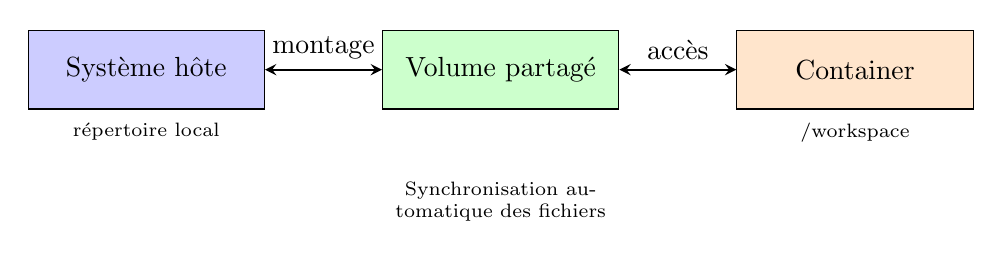
\begin{tikzpicture}[scale=0.9,
    box/.style={rectangle,draw,minimum width=3cm,minimum height=1cm,align=center},
    arrow/.style={->,>=stealth,thick}]

\node[box,fill=blue!20] (host) at (0,0) {Système hôte};
\node[below=0.05cm of host,font=\scriptsize] {répertoire local};

\node[box,fill=green!20] (vol) at (5,0) {Volume partagé};

\node[box,fill=orange!20] (cont) at (10,0) {Container};
\node[below=0.05cm of cont,font=\scriptsize] {/workspace};

\draw[arrow,<->] (host) -- (vol) node[midway,above] {montage};
\draw[arrow,<->] (vol) -- (cont) node[midway,above] {accès};

\node[below=0.8cm of vol,text width=4cm,font=\scriptsize,align=center] {Synchronisation automatique des fichiers};

\end{tikzpicture}
\end{center}

\subsection{Navigation dans le Container}

Une fois dans le container, vous êtes dans un système Linux minimal.

\begin{techbox}{Commandes de base Linux}
\begin{verbatim}
# Vérifier le répertoire courant (vous êtes déjà dans /workspace)
pwd

# Lister les fichiers
ls -la

# Créer un répertoire
mkdir mon_projet

# Quitter le container
exit
\end{verbatim}
\end{techbox}

\section{Prise en Main de Vim}

\begin{warningbox}{Vim est obligatoire dans ce cours}
\textbf{Vim est l'éditeur OBLIGATOIRE pour tout le cours de Programmation C Avancée.}

Tous les TPs supposent que vous utilisez Vim. Cette contrainte n'est pas arbitraire :
\begin{itemize}
\item Vim est présent sur tous les systèmes Unix/Linux (serveurs, systèmes embarqués)
\item Compétence essentielle pour un ingénieur système
\item Productivité maximale une fois maîtrisé
\item Préparation aux situations professionnelles sans interface graphique
\end{itemize}

\textbf{vs. code (ou nano) est disponible pour dépannage uniquement.} Toutes les instructions de TP utilisent Vim.
\end{warningbox}

Dans le container Docker, \textbf{Vim} est l'éditeur de texte à maîtriser. Cette section vous guide à travers les opérations essentielles d'un programmeur C.

\begin{infobox}{Vim en 3 concepts}
\textbf{1. Modes:} Vim a plusieurs modes. Le plus important: \texttt{ESC} revient toujours au mode NORMAL.

\textbf{2. Mode INSERT:} Pour taper du texte, appuyer sur \texttt{i}. Pour sortir, appuyer sur \texttt{ESC}.

\textbf{3. Commandes:} En mode NORMAL, taper \texttt{:wq} puis ENTER pour sauvegarder et quitter.
\end{infobox}

\begin{exercicebox}{Exercice 1: Premiers pas avec Vim}
\textbf{Objectif:} Créer et éditer un fichier C avec les opérations de base.

\textbf{Étape 1:} Dans le container, créer un fichier:
\begin{verbatim}
vim hello.c
\end{verbatim}

Vim s'ouvre en mode NORMAL (vous ne pouvez pas taper de texte).

\textbf{Étape 2:} Passer en mode INSERT pour taper du code:
\begin{itemize}
\item Appuyer sur \texttt{i}
\item En bas, vous voyez \texttt{-- INSERT --}
\item Taper exactement ce code:
\end{itemize}

\begin{lstlisting}[language=C]
#include <stdio.h>

int main() {
printf("Hello World\n");
return 0;
}
\end{lstlisting}

\textbf{Étape 3:} Sauvegarder et quitter:
\begin{itemize}
\item Appuyer sur \texttt{ESC} (revenir au mode NORMAL)
\item Taper \texttt{:wq} puis ENTER
\end{itemize}

\textbf{Étape 4:} Vérifier que le fichier existe:
\begin{verbatim}
cat hello.c
gcc hello.c -o hello
./hello
\end{verbatim}

Si vous voyez "Hello World", bravo ! Vous avez créé votre premier fichier avec Vim.
\end{exercicebox}

\begin{exercicebox}{Exercice 2: Édition et navigation}
\textbf{Objectif:} Modifier un fichier existant et naviguer dans le code.

\textbf{Étape 1:} Rouvrir le fichier:
\begin{verbatim}
vim hello.c
\end{verbatim}

\textbf{Étape 2:} Navigation (en mode NORMAL):
\begin{itemize}
\item \texttt{j} pour descendre, \texttt{k} pour monter
\item \texttt{h} pour gauche, \texttt{l} pour droite
\item \texttt{gg} pour aller au début du fichier
\item \texttt{G} pour aller à la fin
\end{itemize}

Placer le curseur sur la ligne \texttt{printf}.

\textbf{Étape 3:} Ajouter une nouvelle ligne:
\begin{itemize}
\item En mode NORMAL, appuyer sur \texttt{o} (ouvre une ligne EN DESSOUS)
\item Vim passe automatiquement en mode INSERT
\item Taper: \texttt{printf("Vim works!{\textbackslash}n");}
\item Appuyer sur \texttt{ESC}
\end{itemize}

\textbf{Étape 4:} Copier-coller une ligne:
\begin{itemize}
\item Placer le curseur sur une ligne \texttt{printf}
\item En mode NORMAL, taper \texttt{yy} (copier la ligne)
\item Taper \texttt{p} (coller en dessous)
\end{itemize}

\textbf{Étape 5:} Supprimer une ligne:
\begin{itemize}
\item Placer le curseur sur la ligne à supprimer
\item Taper \texttt{dd}
\end{itemize}

\textbf{Étape 6:} Annuler et refaire:
\begin{itemize}
\item \texttt{u} pour annuler (undo)
\item \texttt{Ctrl+r} pour refaire (redo)
\end{itemize}

\textbf{Étape 7:} Corriger l'indentation:
\begin{itemize}
\item Taper \texttt{gg} pour aller au début
\item Taper \texttt{=G} pour auto-indenter tout le fichier
\end{itemize}

\textbf{Étape 8:} Sauvegarder et tester:
\begin{itemize}
\item \texttt{:wq}
\item Compiler: \texttt{gcc hello.c -o hello}
\item Exécuter: \texttt{./hello}
\end{itemize}
\end{exercicebox}

\begin{exercicebox}{Exercice 3: Recherche et remplacement}
\textbf{Objectif:} Rechercher et modifier du texte rapidement.

\textbf{Étape 1:} Créer un fichier avec du code à modifier:
\begin{verbatim}
vim calcul.c
\end{verbatim}

En mode INSERT (\texttt{i}), taper:
\begin{lstlisting}[language=C]
#include <stdio.h>

int main() {
    int x = 10;
    int y = 10;
    int z = x + y;
    printf("Result: %d\n", z);
    return 0;
}
\end{lstlisting}

Sauvegarder: \texttt{ESC} puis \texttt{:wq}

\textbf{Étape 2:} Rouvrir et rechercher:
\begin{verbatim}
vim calcul.c
\end{verbatim}

\begin{itemize}
\item Taper \texttt{/int} puis ENTER (cherche "int")
\item Taper \texttt{n} pour aller à l'occurrence suivante
\item Taper \texttt{N} pour revenir à la précédente
\end{itemize}

\textbf{Étape 3:} Remplacer toutes les occurrences de "10" par "20":
\begin{itemize}
\item Taper \texttt{:\%s/10/20/g} puis ENTER
\item Toutes les valeurs 10 deviennent 20
\end{itemize}

\textbf{Étape 4:} Sauvegarder et tester:
\begin{itemize}
\item \texttt{:wq}
\item \texttt{gcc calcul.c -o calcul \&\& ./calcul}
\end{itemize}
\end{exercicebox}

\begin{warningbox}{Sortir de Vim si vous êtes bloqué}
Si vous ne savez plus quoi faire dans Vim:
\begin{enumerate}
\item Appuyez sur \texttt{ESC} plusieurs fois (revenir au mode NORMAL)
\item Tapez \texttt{:q!} puis ENTER (quitter sans sauvegarder)
\item Ou tapez \texttt{:wq} puis ENTER (sauvegarder et quitter)
\end{enumerate}
\end{warningbox}

\subsection{Tableau Récapitulatif des Commandes Vim}

\begin{center}
\begin{tabular}{|l|l|p{6cm}|}
\hline
\textbf{Catégorie} & \textbf{Commande} & \textbf{Action} \\
\hline
\hline
\multicolumn{3}{|c|}{\textbf{Modes}} \\
\hline
Passer en INSERT & \texttt{i} & Insérer avant le curseur \\
& \texttt{a} & Insérer après le curseur \\
& \texttt{o} & Nouvelle ligne en dessous \\
& \texttt{O} & Nouvelle ligne au dessus \\
Retour NORMAL & \texttt{ESC} & Toujours revenir au mode NORMAL \\
\hline
\hline
\multicolumn{3}{|c|}{\textbf{Navigation}} \\
\hline
Déplacement & \texttt{h j k l} & Gauche, Bas, Haut, Droite \\
& \texttt{w} & Mot suivant \\
& \texttt{b} & Mot précédent \\
Lignes & \texttt{gg} & Début du fichier \\
& \texttt{G} & Fin du fichier \\
& \texttt{:42} & Aller à la ligne 42 \\
Page & \texttt{Ctrl+f} & Page suivante \\
& \texttt{Ctrl+b} & Page précédente \\
\hline
\hline
\multicolumn{3}{|c|}{\textbf{Édition}} \\
\hline
Supprimer & \texttt{x} & Supprimer caractère \\
& \texttt{dd} & Supprimer ligne \\
& \texttt{dw} & Supprimer mot \\
Copier/Coller & \texttt{yy} & Copier ligne \\
& \texttt{p} & Coller après \\
& \texttt{P} & Coller avant \\
Annuler & \texttt{u} & Annuler (undo) \\
& \texttt{Ctrl+r} & Refaire (redo) \\
\hline
\hline
\multicolumn{3}{|c|}{\textbf{Recherche}} \\
\hline
Chercher & \texttt{/motif} & Chercher vers le bas \\
& \texttt{?motif} & Chercher vers le haut \\
& \texttt{n} & Occurrence suivante \\
& \texttt{N} & Occurrence précédente \\
Remplacer & \texttt{:s/old/new/} & Remplacer sur la ligne \\
& \texttt{:\%s/old/new/g} & Remplacer dans tout le fichier \\
\hline
\hline
\multicolumn{3}{|c|}{\textbf{Sauvegarder/Quitter}} \\
\hline
Fichier & \texttt{:w} & Sauvegarder \\
& \texttt{:q} & Quitter \\
& \texttt{:wq} ou \texttt{:x} & Sauvegarder et quitter \\
& \texttt{:q!} & Quitter sans sauvegarder \\
\hline
\hline
\multicolumn{3}{|c|}{\textbf{Spécial C}} \\
\hline
Indentation & \texttt{>>} & Indenter ligne \\
& \texttt{<<} & Dés-indenter ligne \\
& \texttt{gg=G} & Auto-indenter tout le fichier \\
Navigation code & \texttt{\%} & Aller à l'accolade/parenthèse correspondante \\
\hline
\end{tabular}
\end{center}

\begin{infobox}{Pour aller plus loin}
Si vous voulez approfondir Vim, le container inclut le tutoriel interactif:
\begin{verbatim}
vimtutor
\end{verbatim}
Ce tutoriel de 25-30 minutes couvre toutes les bases de manière interactive.
\end{infobox}

\section{Premier Programme C}

\begin{exercicebox}{Exercice 1: Hello World}
\textbf{Objectif:} Compiler et exécuter un programme C dans le container.

\textbf{Étape 1:} Sur votre système (pas dans Docker), créer un répertoire pour le TP:
\begin{verbatim}
mkdir tp_setup
cd tp_setup
\end{verbatim}

\textbf{Étape 2:} Créer un fichier \texttt{hello.c} avec votre éditeur préféré:
\begin{lstlisting}[language=C]
#include <stdio.h>

int main() {
    printf("Hello from Docker container!\n");
    printf("Compilation successful!\n");
    return 0;
}
\end{lstlisting}

\textbf{Étape 3:} Lancer le container Docker depuis le répertoire \texttt{tp\_setup}.

\textbf{Étape 4:} Dans le container:
\begin{verbatim}
gcc -Wall -Wextra -o hello hello.c
./hello
\end{verbatim}

\textbf{Résultat attendu:}
\begin{verbatim}
Hello from Docker container!
Compilation successful!
\end{verbatim}
\end{exercicebox}

\begin{exercicebox}{Exercice 2: Vérification des outils}
\textbf{Objectif:} Tester tous les outils disponibles dans le container.

\textbf{2.1) Compiler avec warnings stricts:}
\begin{verbatim}
gcc -Wall -Wextra -pedantic -std=c11 hello.c -o hello
\end{verbatim}

\textbf{2.2) Vérifier la version des outils:}
\begin{verbatim}
gcc --version
gdb --version
make --version
valgrind --version
\end{verbatim}

\textbf{2.3) Tester GDB:}
\begin{verbatim}
gcc -g hello.c -o hello_debug
gdb ./hello_debug
(gdb) break main
(gdb) run
(gdb) next
(gdb) print "GDB works!"
(gdb) quit
\end{verbatim}

\textbf{2.4) Tester Valgrind:}
\begin{verbatim}
valgrind ./hello
\end{verbatim}

Vous devriez voir un rapport sans erreurs mémoire.
\end{exercicebox}

\section{Création d'un Makefile}

\begin{exercicebox}{Exercice 3: Makefile de base}
\textbf{Objectif:} Automatiser la compilation avec Make.

Créer un fichier \texttt{Makefile} (attention à la casse):
\begin{lstlisting}[language=make]
# Variables
CC = gcc
CFLAGS = -Wall -Wextra -std=c11 -g
LDFLAGS =

# Cibles
TARGETS = hello

# Regle par defaut
all: $(TARGETS)

# Compilation de hello
hello: hello.c
	$(CC) $(CFLAGS) -o hello hello.c $(LDFLAGS)

# Nettoyage
clean:
	rm -f $(TARGETS) *.o

# Recompilation complete
rebuild: clean all

# Marquer les cibles comme phoniques
.PHONY: all clean rebuild
\end{lstlisting}

\textbf{Utilisation:}
\begin{verbatim}
make              # Compile
make clean        # Nettoie
make rebuild      # Recompile tout
\end{verbatim}

\textbf{Test:} Modifier \texttt{hello.c}, puis taper simplement \texttt{make}.
\end{exercicebox}



\section{Validation de l'Installation}

\begin{exercicebox}{Exercice 4: Test complet}
\textbf{Objectif:} Valider que tout fonctionne correctement.

Créer un programme \texttt{test\_env.c}:
\begin{lstlisting}[language=C]
#include <stdio.h>
#include <stdlib.h>

int main() {
    printf("=== Test Environnement ===\n");
    
    // Test 1: Compilation
    printf("[OK] Compilation reussie\n");
    
    // Test 2: Allocation memoire
    int *ptr = malloc(10 * sizeof(int));
    if (ptr != NULL) {
        printf("[OK] malloc fonctionne\n");
        free(ptr);
    }
    
    // Test 3: Arithmetique
    int result = 42 + 27;
    if (result == 69) {
        printf("[OK] Arithmetique correcte\n");
    }
    
    printf("\nEnvironnement pret pour le cours!\n");
    return 0;
}
\end{lstlisting}

\textbf{Compiler et exécuter:}
\begin{verbatim}
gcc -Wall -Wextra -g test_env.c -o test_env
./test_env
valgrind --leak-check=full ./test_env
\end{verbatim}

\textbf{Résultat attendu:}
\begin{itemize}
\item Tous les tests [OK]
\item Valgrind ne rapporte aucune fuite mémoire
\end{itemize}

Si tous les tests passent, votre environnement est correctement configuré!
\end{exercicebox}

\section*{Conclusion}

Vous avez maintenant un environnement de développement C professionnel et standardisé. Cet environnement sera utilisé pour tous les TP du cours.

\begin{infobox}{Points clés à retenir}
\begin{itemize}
\item Toujours lancer Docker depuis le répertoire de travail
\item Éditer les fichiers sur votre système, compiler dans Docker
\item Utiliser \texttt{make} pour automatiser la compilation
\item GDB et Valgrind sont vos amis pour le debugging
\end{itemize}
\end{infobox}


\end{document}